\documentclass{article}
% setup page
\usepackage[utf8]{inputenc}
\usepackage{fancyhdr}
\usepackage[a4paper, top=2.5cm, left=2cm, right=2cm, bottom=2cm]{geometry}
\usepackage{titling}

% for random text
\usepackage{lipsum}

\usepackage{todonotes}
\usepackage{amsmath}
\usepackage{graphics}

\usepackage[backend=bibtex]{biblatex}
\addbibresource{papers.bib}

% setup info
\title{IR Project 1: Report}
\author{Tobias Veto, Philip Junker, Marc Fischer}

% setup header/footer
\pagestyle{fancy}
\fancyhf{}
\rhead{\theauthor}
\lhead{\thetitle}
\rfoot{Page \thepage}
 

\begin{document}

\section*{TODO}
\begin{itemize}
	\item result files
	\item readme file
	\item package code and results
	\item finish report
	\item clean up bibtex notes
\end{itemize}

 
\section*{Introduction}
For the implementations of the naive bayes, logistic regession and SVM we stayed close to the code shown in the lecture. Thus the implementations of the algorithms were straightforward while optimization and data preprocessing were challenging. Most of our effort went into the data pruning.

In our team one person each focues on one classifier. While we shared insights, and the code that we use for the reader, this might account for inconsitencies in the code and different tone in the chapters of this report.


\section*{Data transformation and pruning}
A big part of our implementation was data preprocessing. We read the tokens from the documents (with tinyIR), remove tokens not consiting of letters, stem the word and remove stopwords. \cite{joachims_text_1998,ozgur_text_2005} both list this as the standard approach to preprocessing in document classifcation. From the resulting corpus of documents we remove those that occur less then \texttt{minOccurrence} and those that are found in more than $\text{\texttt{maxOccurrenceRate}} \cdot \text{\texttt{nrDocuments}}$, where $\text{\texttt{maxOccurrenceRate}} \in (0, 1]$.
The resulting dictionary of words is uses to rerpresent each document as a bag-of-words vector. For the weights within the vector we use boolean weights (1 if the word occurs in the document, else 0), tf-idf weights (insprired by \cite{ozgur_text_2005}) and the count of word.  \todo{specify weighting method here} has generally yielded the best result.
We also discovered, that words extracted from the title of the document contain a high amount of information and lend themselves especially to predicting country codes. The words from the titles were processed like the words from the content.

We also tied to access the data in a random order. Our assumption was that some classes might only show up at the end of the stream of documents and thus, might only be encountert with a very low learning rate (in Logistic Rergession and SVM).
However, the random ofer had only neglicbale effects on the performance of the algorithms. As the order is irrelevant for the Naive Bayes approach, this has no impact on it.

\section*{Naive Bayes}
We used the formulas for Naive Bayes as shown in the lecture. For each code we calculated the probability $P(word | code)$ for every word in the reduced dictionary.
For each of the three different code-types a different threshold was evaluated. The advantage of this approach is the independence of the code-types and therefore the possibility of a country-code to be predicted although the probability for this code given a document is much lower than for all the topic-codes. The performance in form of F1-scores is plotted for both country- and topic-codes in figure \ref{fig_bayesThreshold}. Because the industry-codes are very hard to predict the optimal threshold for these codes turned out to be zero, meaning we do never predict an industry code.
While the word-code-probabilities for the topic-codes were calculated using the content of the Reuters-articles we used only the article-titles to calculate the probabilities for the country-codes. 
\begin{figure}[h!]
    \centering
    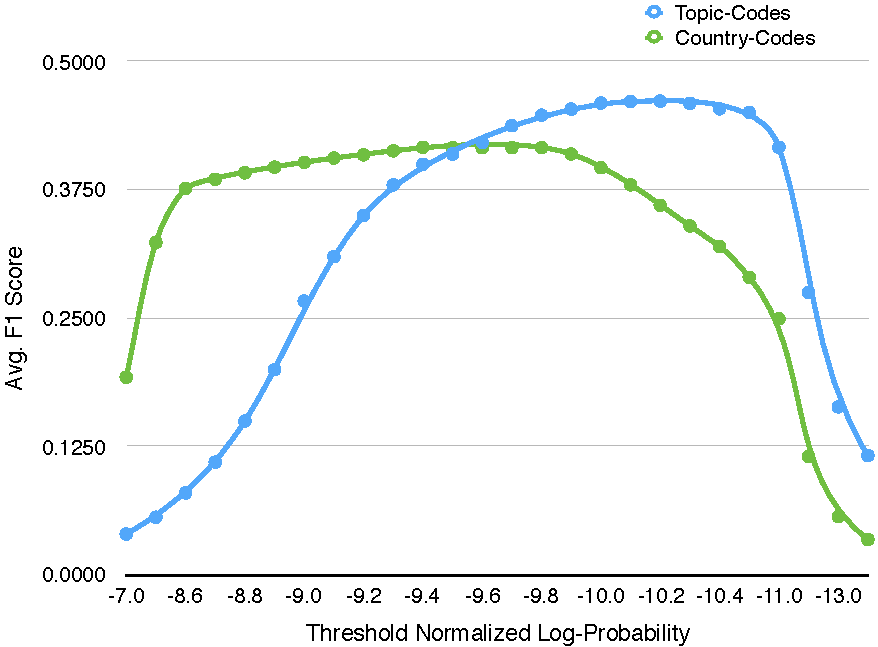
\includegraphics[scale=0.6]{graphics/BayesF1ScoreTopicCountry.pdf}
    \caption{This figure shows the average F1-Score of topic- and country-codes using different thresholds for the normalized log-probability.}
    \label{fig_bayesThreshold}
\end{figure}

\section*{Logistic Regression}
\lipsum[1-4] %replace with real text

\section*{SVM}
The algorithm shown in the lecture is the well-known pegsasos algorithm\cite{shalev-shwartz_pegasos:_2011,shalev-shwartz_pegasos:_????}. For the implementation we train one SVM per category occuring in the training data in an all-vs-one approach.
Data was preproccessed as introduced before with the use of homogeneous coordinates (bias term) and without. The listed papers suggest, not using a bias with the normal formulation of the pegasos algorith or to adjust it if doing so, as it undermines the convergences guarantee. However we see a slight increase in performance if using homogenous coordinates and the SVM formulation form the lecture.
The results from \cite{joachims_text_1998} strongly suggest to use a polynomial or RBF kernel, but \todo{RBF on title}.


The SVM achieves very high prcesision, but poor recall indincating that it is too strict (not giving labels that should be there). Lowering the $\lambda$ parameter could solve this. If this still does not solve it, it might indicate a non-linearly sperable set. This would suggest the usage of kernels.


\printbibliography

\end{document}